% preamble-exam-zh.tex — 共享 preamble
% 用于所有 exam-zh 模板
%
% 样式策略：
%   屏幕 → 语义彩色（蓝=关键想法，红=易错，绿=路线，灰=提示/教师备注）
%   打印 → 自动降级为黑白（通过 print mode 或 monochrome 选项）

\documentclass{exam-zh}

% ---------- 基础配置 ----------
\examsetup{
  page/size = a4paper,
  page/show-head = false,
  page/show-foot = false,
  sealline/show = false,
  font = times,
  math-font = xits,
}

\usepackage{tcolorbox}
\usepackage{needspace}
\usepackage{graphicx}
\usepackage{tikz}
\usetikzlibrary{calc,intersections,angles,quotes,arrows.meta,decorations.markings,patterns.meta,backgrounds}
\usepackage{pgfplots}
\pgfplotsset{compat=1.18}
\tcbuselibrary{skins,breakable}

% ---------- 打印/屏幕颜色切换 ----------
% 用法：\documentclass[monochrome]{exam-zh} 即可切换为纯黑白
% 注意：不要使用 \if@xxx 放在 makeatother 外部；这里改成普通条件名。
\newif\ifeduprintcolor
\eduprintcolortrue

\makeatletter
\@ifclasswith{exam-zh}{monochrome}{\eduprintcolorfalse}{}
\makeatother

% ---------- 语义颜色定义 ----------
% 屏幕：有色彩区分；打印：降级为灰度
\ifeduprintcolor
  % --- 屏幕彩色模式 ---
  \definecolor{edu-blue}{RGB}{47, 82, 122}       % 关键想法
  \definecolor{edu-blue-bg}{RGB}{243, 246, 252}
  \definecolor{edu-red}{RGB}{180, 40, 40}         % 易错提醒
  \definecolor{edu-red-bg}{RGB}{255, 245, 240}
  \definecolor{edu-green}{RGB}{34, 100, 60}       % 路线图
  \definecolor{edu-green-bg}{RGB}{242, 250, 245}
  \definecolor{edu-orange}{RGB}{160, 90, 0}       % 训练目标
  \definecolor{edu-orange-bg}{RGB}{255, 248, 235}
  \definecolor{edu-gray}{RGB}{100, 100, 100}      % 提示/教师备注
  \definecolor{edu-gray-bg}{RGB}{248, 248, 248}
  \definecolor{edu-purple}{RGB}{90, 50, 120}      % 思考题
  \definecolor{edu-purple-bg}{RGB}{248, 244, 252}
\else
  % --- 打印黑白模式 ---
  \definecolor{edu-blue}{gray}{0.15}
  \definecolor{edu-blue-bg}{gray}{0.96}
  \definecolor{edu-red}{gray}{0.25}
  \definecolor{edu-red-bg}{gray}{0.97}
  \definecolor{edu-green}{gray}{0.20}
  \definecolor{edu-green-bg}{gray}{0.97}
  \definecolor{edu-orange}{gray}{0.25}
  \definecolor{edu-orange-bg}{gray}{0.98}
  \definecolor{edu-gray}{gray}{0.40}
  \definecolor{edu-gray-bg}{gray}{0.97}
  \definecolor{edu-purple}{gray}{0.30}
  \definecolor{edu-purple-bg}{gray}{0.98}
\fi
\colorlet{edu-diagram-muted}{edu-gray}
\providecommand{\edukai}{\kaishu}

% ---------- TikZ diagram semantic macros ----------
\definecolor{edu-diagram-ink}{RGB}{17,24,39}
\definecolor{edu-diagram-marker}{RGB}{220,38,38}
\definecolor{edu-diagram-angle}{RGB}{5,150,105}
\tikzset{
  diagram point/.style={fill=edu-diagram-ink},
  diagram tick/.style={draw=edu-diagram-marker,line width=0.9pt,line cap=round},
  diagram segment/.style={draw=edu-diagram-ink,line cap=round},
  point label/.style={inner sep=1pt},
  condition label/.style={inner sep=1pt}
}
\providecommand{\DrawSegment}[3][]{\draw[diagram segment,#1] (#2) -- (#3);}
\providecommand{\DrawDashedSegment}[3][]{\draw[diagram segment,dashed,#1] (#2) -- (#3);}
\providecommand{\Triangle}[4][]{\path[#1] (#2) -- (#3) -- (#4) -- cycle;}
\providecommand{\Quadrilateral}[5][]{\path[#1] (#2) -- (#3) -- (#4) -- (#5) -- cycle;}
\providecommand{\PolygonPath}[2][]{\path[#1] #2 -- cycle;}
\providecommand{\DiagramPointRadius}{0.052cm}
\providecommand{\PointDot}[2][]{\fill[diagram point,#1] (#2) circle[radius=\DiagramPointRadius];}
\providecommand{\PointLabel}[3][]{\node[point label,#1] at (#2) {#3};}
\providecommand{\SegmentLabel}[4][]{\node[condition label,#1] at ($(#2)!0.5!(#3)$) {#4};}
\providecommand{\CoordinateTag}[3][]{\node[condition label,#1] at (#2) {#3};}
\providecommand{\AngleMark}[4][]{\pic[draw=edu-diagram-angle,line width=0.9pt,angle radius=0.48cm,#1] {angle=#2--#3--#4};}
\providecommand{\AngleLabel}[5][]{\pic["{#5}",draw=none,angle radius=0.64cm,#1] {angle=#2--#3--#4};}
\providecommand{\RightAngleMark}[4][]{\pic[draw=edu-diagram-marker,line width=0.9pt,angle radius=0.28cm,#1] {right angle=#2--#3--#4};}
\providecommand{\EqualTick}[3][]{%
  \path[postaction={decorate},decoration={markings,mark=at position .5 with {\draw[diagram tick,#1] (0pt,-4pt) -- (0pt,4pt);}}] (#2) -- (#3);%
}
\providecommand{\DoubleEqualTick}[3][]{%
  \path[postaction={decorate},decoration={markings,mark=at position .46 with {\draw[diagram tick,#1] (0pt,-4pt) -- (0pt,4pt);},mark=at position .54 with {\draw[diagram tick,#1] (0pt,-4pt) -- (0pt,4pt);}}] (#2) -- (#3);%
}
\providecommand{\TripleEqualTick}[3][]{%
  \path[postaction={decorate},decoration={markings,mark=at position .43 with {\draw[diagram tick,#1] (0pt,-4pt) -- (0pt,4pt);},mark=at position .5 with {\draw[diagram tick,#1] (0pt,-4pt) -- (0pt,4pt);},mark=at position .57 with {\draw[diagram tick,#1] (0pt,-4pt) -- (0pt,4pt);}}] (#2) -- (#3);%
}
\providecommand{\ParallelMark}[3][]{\EqualTick[#1]{#2}{#3}}
\providecommand{\NamedSegmentPath}[3]{\path[name path=#1] (#2) -- (#3);}
\providecommand{\IntersectPaths}[3]{\path[name intersections={of=#2 and #3, by=#1}];}

% ---------- 自定义教学环境 ----------
% 共性：enhanced + breakable（跨页不断裂）

% 原题卡片 — 强边框，突出显示
\newtcolorbox{problemcard}{
  enhanced, breakable,
  colback=edu-blue-bg,
  colframe=edu-blue,
  boxrule=1.2pt,
  arc=0pt,
  left=3mm, right=3mm, top=3mm, bottom=3mm,
}

% 解题路线图 — 左边线 + 浅底
\newtcolorbox{routebox}{
  enhanced, breakable,
  colback=edu-green-bg,
  colframe=edu-green!30,
  boxrule=0pt,
  borderline west={2.5pt}{0pt}{edu-green},
  left=3mm, right=3mm, top=3mm, bottom=3mm,
}

% 关键想法 — 蓝色左边线
\newtcolorbox{keyideabox}{
  enhanced, breakable,
  colback=edu-blue-bg,
  colframe=edu-blue!30,
  boxrule=0pt,
  borderline west={2.5pt}{0pt}{edu-blue},
  left=3mm, right=3mm, top=3mm, bottom=3mm,
}

% 易错提醒 — 红色左边线
\newtcolorbox{mistakebox}{
  enhanced, breakable,
  colback=edu-red-bg,
  colframe=edu-red!20,
  boxrule=0pt,
  borderline west={3pt}{0pt}{edu-red},
  left=3mm, right=3mm, top=2.5mm, bottom=2.5mm,
}

% 提示 — 灰色虚线左边线
\newtcolorbox{hintbox}{
  enhanced, breakable,
  colback=edu-gray-bg,
  colframe=edu-gray!20,
  boxrule=0pt,
  borderline west={2pt}{0pt}{edu-gray, dashed},
  left=3mm, right=3mm, top=2mm, bottom=2mm,
  fontupper=\edukai\small,
}

% 思考题 — 紫色虚线左边线
\newtcolorbox{thinkbox}{
  enhanced, breakable,
  colback=edu-purple-bg,
  colframe=edu-purple!20,
  boxrule=0pt,
  borderline west={2pt}{0pt}{edu-purple, dashed},
  left=2.5mm, right=2.5mm, top=2.5mm, bottom=2.5mm,
}

% 教师备注 — 灰色左边线，小字
\newtcolorbox{teachernote}{
  enhanced, breakable,
  colback=edu-gray-bg,
  colframe=edu-gray!15,
  boxrule=0pt,
  borderline west={2pt}{0pt}{edu-gray!60},
  left=2.5mm, right=2.5mm, top=2.5mm, bottom=2.5mm,
  fontupper=\small,
  colupper=black!60,
}

% 训练目标 — 橙色左边线，小字
\newtcolorbox{traininggoal}{
  enhanced, breakable,
  colback=edu-orange-bg,
  colframe=edu-orange!15,
  boxrule=0pt,
  borderline west={1.5pt}{0pt}{edu-orange},
  left=2mm, right=2mm, top=1mm, bottom=1mm,
  fontupper=\small,
}

% 答题区 — 无边框，纯留白
\newcommand{\answerarea}[1][40mm]{%
  \vspace{2mm}%
  \begin{tcolorbox}[
    enhanced, breakable,
    colback=white,
    colframe=white,
    boxrule=0pt,
    height=#1,
    valign=top,
    bottom=0mm,
    after skip=0mm,
  ]
  \end{tcolorbox}%
}

\newsavebox{\diagramtikzbox}

\newenvironment{diagramcoltikz}[2]{%
  \begin{minipage}[t]{#1}
    \vspace{0pt}\centering
    \def\diagramcaption{#2}%
    \begin{lrbox}{\diagramtikzbox}%
}{%
    \end{lrbox}%
    \usebox{\diagramtikzbox}%
    \ifx\diagramcaption\empty\else
      \par\vspace{1mm}{\scriptsize\color{edu-diagram-muted}\diagramcaption}
    \fi
  \end{minipage}%
}

\newenvironment{diagramrowtikz}[3]{%
  \begin{minipage}[t]{#1}
    \vspace{0pt}\centering
    \def\diagramlabel{#2}%
    \def\diagramcaption{#3}%
    \begin{lrbox}{\diagramtikzbox}%
}{%
    \end{lrbox}%
    \usebox{\diagramtikzbox}%
    \ifx\diagramlabel\empty\else
      \par\vspace{1mm}{\scriptsize\bfseries\diagramlabel}
    \fi
    \ifx\diagramcaption\empty\else
      \par\vspace{0.5mm}{\scriptsize\color{edu-diagram-muted}\diagramcaption}
    \fi
  \end{minipage}%
}

\newenvironment{answerareawithdiagramtikz}[3]{%
  \par\vspace{2mm}%
  \noindent
  \begin{minipage}[t]{\dimexpr\linewidth-#2-6mm\relax}
    \vspace{0pt}\rule{0pt}{#1}
  \end{minipage}\hfill
  \begin{diagramcoltikz}{#2}{#3}
}{%
  \end{diagramcoltikz}
  \par\vspace{2mm}%
}

% ---------- 字体设置 ----------
% exam-zh (ctexbook) already sets CJK fonts via ctex.
% Only override if specific fonts are needed.
% macOS: Songti SC, STHeiti, STFangsong
% Linux: SimSun, SimHei, FangSong

% ---------- 页面设置 ----------
% exam-zh (ctexbook) already loads geometry.
% Override margins if needed:
% \geometry{top=16mm, bottom=16mm, left=14mm, right=14mm}

\examsetup{
  question/show-answer = true,
  fillin/show-answer = true,
  solution/show-solution = show-stay,
}

% ---------- 教师版解答样式 ----------
\newtcolorbox{solutionblock}{
  enhanced, breakable,
  colback=edu-blue-bg,
  colframe=edu-blue!25,
  boxrule=0pt,
  borderline west={2pt}{0pt}{edu-blue!50},
  arc=0pt,
  left=3mm, right=3mm, top=2mm, bottom=2mm,
  before skip=2mm,
  after skip=3mm,
  fontupper=\small,
}

% 解答步骤编号
\newcounter{solstep}
\newcommand{\solstep}[2]{%
  \stepcounter{solstep}%
  \par\medskip
  \noindent\hangindent=6mm
  {\color{edu-blue}\bfseries\textcircled{\scriptsize\thesolstep}\enspace #1}\enspace #2\par
}

\begin{document}

\section*{线段比再练（教师版）}

\section*{一、线段比练习（每题 8 分，共 48 分）}

\needspace{8\baselineskip}

\begin{problem}[points=8]
  \noindent
  \begin{minipage}[t]{\dimexpr\linewidth-64mm-6mm\relax}
    \vspace{0pt}
    点 $A,B,C$ 在同一直线上，顺序为 $A-B-C$。若 $AB:BC=3:5$，且 $AC=64$，求 $BC$。

    \begin{hintbox}
\textbf{提示：}要求 $BC$，已知 $AC$，先想 $BC:AC$。\par 再把 $AC$ 改成总份数 $3+5$。\end{hintbox}

  \end{minipage}\hfill
  \begin{diagramcoltikz}{64mm}{第 1 题图}
  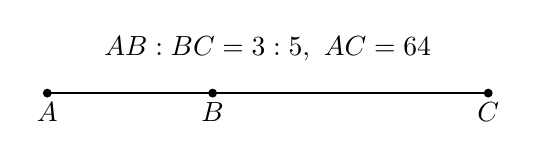
\begin{tikzpicture}[x=1cm,y=1cm,baseline=(current bounding box.center)]
  \draw[line width=1pt] (0,0) -- (5.6,0);
  \fill (0,0) circle (1.6pt) node[below] {$A$};
  \fill (2.1,0) circle (1.6pt) node[below] {$B$};
  \fill (5.6,0) circle (1.6pt) node[below] {$C$};
  \node[above=8pt] at (2.8,0) {$AB:BC=3:5,\ AC=64$};
\end{tikzpicture}
  \end{diagramcoltikz}
  \par\medskip
  \answerarea[30mm]
  \setcounter{solstep}{0}
  \begin{solutionblock}
    \textbf{答案：}$BC=40$\par\medskip
    \solstep{先定目标比}{题目要求 $BC$，已知 $AC$，所以先定 $BC:AC$。}
    \solstep{改成可比较的份数}{$AB:BC=3:5$，$AC$ 共 $3+5=8$ 份，所以 $BC:AC=5:8$。}
    \solstep{乘已知量}{$BC=64\times\dfrac{5}{8}=40$。}
  \end{solutionblock}
\end{problem}


\needspace{8\baselineskip}

\begin{problem}[points=8]
  \noindent
  \begin{minipage}[t]{\dimexpr\linewidth-64mm-6mm\relax}
    \vspace{0pt}
    点 $A,B,C$ 在同一直线上，顺序为 $A-B-C$。若 $4AB=7BC$，且 $AC=55$，求 $AB$。

    \begin{hintbox}
\textbf{提示：}先把 $4AB=7BC$ 改成线段比。\par 乘法式里，份数和系数是交叉对应的。\end{hintbox}

  \end{minipage}\hfill
  \begin{diagramcoltikz}{64mm}{第 2 题图}
  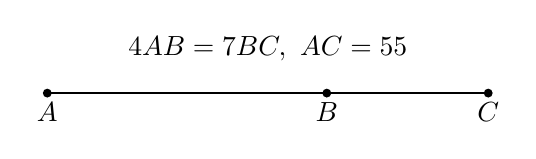
\begin{tikzpicture}[x=1cm,y=1cm,baseline=(current bounding box.center)]
  \draw[line width=1pt] (0,0) -- (5.6,0);
  \fill (0,0) circle (1.6pt) node[below] {$A$};
  \fill (3.55,0) circle (1.6pt) node[below] {$B$};
  \fill (5.6,0) circle (1.6pt) node[below] {$C$};
  \node[above=8pt] at (2.8,0) {$4AB=7BC,\ AC=55$};
\end{tikzpicture}
  \end{diagramcoltikz}
  \par\medskip
  \answerarea[30mm]
  \setcounter{solstep}{0}
  \begin{solutionblock}
    \textbf{答案：}$AB=35$\par\medskip
    \solstep{方程改比例}{$4AB=7BC$，所以 $AB:BC=7:4$。}
    \solstep{目标比}{$AC=AB+BC$，共 $7+4=11$ 份，故 $AB:AC=7:11$。}
    \solstep{求值}{$AB=55\times\dfrac{7}{11}=35$。}
  \end{solutionblock}
\end{problem}


\needspace{8\baselineskip}

\begin{problem}[points=8]
  \noindent
  \begin{minipage}[t]{\dimexpr\linewidth-68mm-6mm\relax}
    \vspace{0pt}
    点 $A,B,C,D$ 在同一直线上，顺序为 $A-B-C-D$。若 $AB:BC:CD=2:3:4$，且 $AD=72$，求 $BD$。

    \begin{hintbox}
\textbf{提示：}$BD$ 是从 $B$ 到 $D$，包含 $BC$ 和 $CD$。\par 把 $BD$ 的份数和 $AD$ 的总份数相比。\end{hintbox}

  \end{minipage}\hfill
  \begin{diagramcoltikz}{68mm}{第 3 题图}
  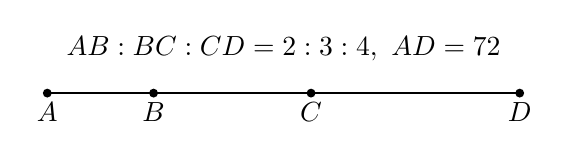
\begin{tikzpicture}[x=1cm,y=1cm,baseline=(current bounding box.center)]
  \draw[line width=1pt] (0,0) -- (6.0,0);
  \fill (0,0) circle (1.6pt) node[below] {$A$};
  \fill (1.35,0) circle (1.6pt) node[below] {$B$};
  \fill (3.35,0) circle (1.6pt) node[below] {$C$};
  \fill (6.0,0) circle (1.6pt) node[below] {$D$};
  \node[above=8pt] at (3.0,0) {$AB:BC:CD=2:3:4,\ AD=72$};
\end{tikzpicture}
  \end{diagramcoltikz}
  \par\medskip
  \answerarea[32mm]
  \setcounter{solstep}{0}
  \begin{solutionblock}
    \textbf{答案：}$BD=56$\par\medskip
    \solstep{看点的顺序}{顺序为 $A-B-C-D$，所以 $BD$ 包含 $BC$ 与 $CD$。}
    \solstep{改份数}{$BD$ 是 $3+4=7$ 份，$AD$ 是 $2+3+4=9$ 份。}
    \solstep{乘已知量}{$BD=72\times\dfrac{7}{9}=56$。}
  \end{solutionblock}
\end{problem}


\needspace{8\baselineskip}

\begin{problem}[points=8]
  \noindent
  \begin{minipage}[t]{\dimexpr\linewidth-64mm-6mm\relax}
    \vspace{0pt}
    点 $A,B,C$ 在同一直线上，顺序为 $A-B-C$。若 $AB:BC=5:7$，且 $AB=30$，求 $AC$。

    
  \end{minipage}\hfill
  \begin{diagramcoltikz}{64mm}{第 4 题图}
  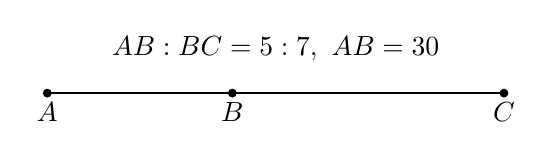
\begin{tikzpicture}[x=1cm,y=1cm,baseline=(current bounding box.center)]
  \draw[line width=1pt] (0,0) -- (5.8,0);
  \fill (0,0) circle (1.6pt) node[below] {$A$};
  \fill (2.35,0) circle (1.6pt) node[below] {$B$};
  \fill (5.8,0) circle (1.6pt) node[below] {$C$};
  \node[above=8pt] at (2.9,0) {$AB:BC=5:7,\ AB=30$};
\end{tikzpicture}
  \end{diagramcoltikz}
  \par\medskip
  \answerarea[30mm]
  \setcounter{solstep}{0}
  \begin{solutionblock}
    \textbf{答案：}$AC=72$\par\medskip
    \solstep{定比较对象}{题目已知 $AB=30$，要求 $AC$，所以用 $AC:AB$ 或 $AB:AC$。}
    \solstep{写比例}{$AB:AC=5:12$。}
    \solstep{求整体}{$AC=30\times\dfrac{12}{5}=72$。}
  \end{solutionblock}
\end{problem}


\needspace{8\baselineskip}

\begin{problem}[points=8]
  \noindent
  \begin{minipage}[t]{\dimexpr\linewidth-68mm-6mm\relax}
    \vspace{0pt}
    点 $A,B,C,D$ 在同一直线上，顺序为 $A-B-C-D$。若 $AB:BC:CD=4:6:5$，且 $AD=75$，求 $AC$。

    
  \end{minipage}\hfill
  \begin{diagramcoltikz}{68mm}{第 5 题图}
  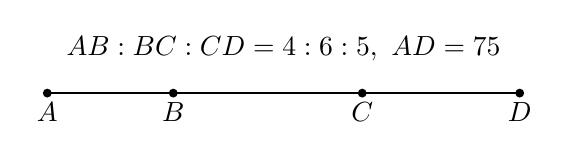
\begin{tikzpicture}[x=1cm,y=1cm,baseline=(current bounding box.center)]
  \draw[line width=1pt] (0,0) -- (6.0,0);
  \fill (0,0) circle (1.6pt) node[below] {$A$};
  \fill (1.6,0) circle (1.6pt) node[below] {$B$};
  \fill (4.0,0) circle (1.6pt) node[below] {$C$};
  \fill (6.0,0) circle (1.6pt) node[below] {$D$};
  \node[above=8pt] at (3.0,0) {$AB:BC:CD=4:6:5,\ AD=75$};
\end{tikzpicture}
  \end{diagramcoltikz}
  \par\medskip
  \answerarea[30mm]
  \setcounter{solstep}{0}
  \begin{solutionblock}
    \textbf{答案：}$AC=50$\par\medskip
    \solstep{目标拆段}{顺序为 $A-B-C-D$，所以 $AC=AB+BC$。}
    \solstep{目标比}{$AC:AD=(4+6):(4+6+5)=10:15=2:3$。}
    \solstep{求值}{$AC=75\times\dfrac{2}{3}=50$。}
  \end{solutionblock}
\end{problem}


\needspace{8\baselineskip}

\begin{problem}[points=8]
  \noindent
  \begin{minipage}[t]{\dimexpr\linewidth-68mm-6mm\relax}
    \vspace{0pt}
    点 $A,B,C,D$ 在同一直线上，顺序为 $A-B-C-D$。若 $AB=18$，$BC:CD=2:5$，且 $AD=81$，求 $CD$。

    
  \end{minipage}\hfill
  \begin{diagramcoltikz}{68mm}{第 6 题图}
  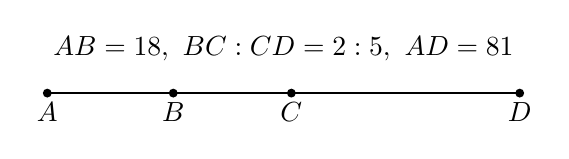
\begin{tikzpicture}[x=1cm,y=1cm,baseline=(current bounding box.center)]
  \draw[line width=1pt] (0,0) -- (6.0,0);
  \fill (0,0) circle (1.6pt) node[below] {$A$};
  \fill (1.6,0) circle (1.6pt) node[below] {$B$};
  \fill (3.1,0) circle (1.6pt) node[below] {$C$};
  \fill (6.0,0) circle (1.6pt) node[below] {$D$};
  \node[above=8pt] at (3.0,0) {$AB=18,\ BC:CD=2:5,\ AD=81$};
\end{tikzpicture}
  \end{diagramcoltikz}
  \par\medskip
  \answerarea[34mm]
  \setcounter{solstep}{0}
  \begin{solutionblock}
    \textbf{答案：}$CD=45$\par\medskip
    \solstep{先改已知量}{$BC:CD$ 只管 $BD$ 这一段，因此先求 $BD=AD-AB=81-18=63$。}
    \solstep{写目标比}{$CD:BD=5:(2+5)=5:7$。}
    \solstep{求值}{$CD=63\times\dfrac{5}{7}=45$。}
  \end{solutionblock}
\end{problem}


\clearpage
\section*{参考答案}


\begin{keyideabox}
  \textbf{线段比再练}
  第 1 题：$BC=40$。
第 2 题：$AB=35$。
第 3 题：$BD=56$。
第 4 题：$AC=72$。
第 5 题：$AC=50$。
第 6 题：$CD=45$。

\end{keyideabox}



\end{document}
